

\begin{figure}[t]
\begin{center}
\scalebox{.67}{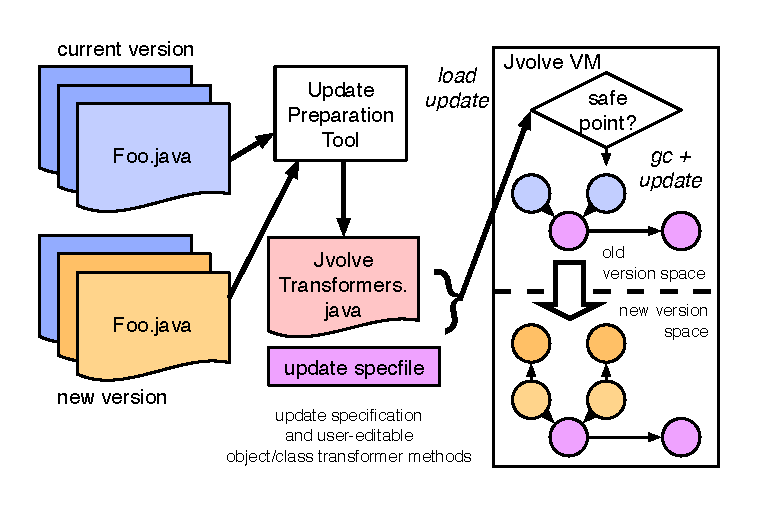
\includegraphics{images/system}}
\end{center}
\caption{Dynamic Software Updating with \DSU}
\label{fig:overview}
\end{figure}


%MWH: I don't think this section is particularly about a VM-centric
%   design.  I've reverted the text back to the way it was.  The next
%   section is about the VM.  We'd have to make more significant
%   changes here, not sure how, to somehow claim this is an overview
%   of VM-centric DSU.  The approach here, modulo the discussion of
%   garbage collection, could just as well apply to a system
%   implemented via rewriting.

% \section{A VM-centric DSU Design}

% This section begins by overviewing a VM-centric approach, our design
% choices, update model, and describes how the developer participates in
% the process. Section~\ref{sec:vm} describes each component in detail.

\section{Dynamic Updates in \DSU}

This section overviews \DSU's approach, what changes it permits, and
how the developer participates in the process.

\subsection{System Overview}
\label{sec:overview}

Figure~\ref{fig:overview} illustrates the dynamic update process.
Assume that the VM is executing the current version of the program,
whose code is depicted in the left top corner.  Meanwhile, developers
prepare a new version and fully test it using standard procedures.
A developer 
then invokes \DSU's \ac{UPT} on the old and
new versions. The \ac{UPT} generates an update specification, which identifies
new and updated classes, and a \texttt{JvolveTransformers.java} file
that contains default \emph{object}
and \emph{class transformer} methods.  

Transformer methods take an
object or class of the old version and 
initialize the corresponding object or class of the new version.  The default
transformers assign default values, such as zero and {\tt null}, to new
instance, reference, and static fields, and copy values for unchanged
fields.  Developers may customize the default transformers as
necessary.  We present an example update and transformer in
Section~\ref{subsec:transformers}. %, and briefly discuss how they are compiled.

The user signals the running VM to apply the update, and the VM loads
the new class files and transformers and schedules the update. The VM
scheduler signals an interrupt, which stops all threads at
VM safe points, where it is safe to perform thread scheduling and garbage collection.  \DSU{} then checks if the VM is % also
at a \emph{DSU safe point}. DSU safe points require that no thread's
activation stack contains a \emph{restricted} method.  Restricted
methods are of three categories: (1) methods changed by the update,
(2) methods whose bytecode is unchanged but whose compiled
representation may change, and (3) methods specified by the user. If
restricted methods are on stack, the VM installs return-barriers
for~(1) and~(3), and performs on-stack-replacement for~(2) to reach a
DSU safe point.  Section~\ref{sec:safe} describes this process in
detail.

Once all application threads have synchronized at DSU safe points, \DSU{}
applies the update. It first invalidates the compiled versions of all
changed methods.
These methods are
recompiled as needed---the adaptive JIT compiler will
generate code the next time the program invokes an invalidated method,
and may optimize it further, if the program executes it frequently.
%
The VM then invokes the
class transformers.  Finally, the VM initiates a full copying garbage collection. It
piggybacks on the garbage collector to detect all existing objects
whose classes change. It allocates objects that conform to the new type
declarations, and performs object transformations to populate the new
objects with valid state. %, as described above.  
At this point, the update is complete.

\begin{figure*}[t]
\begin{tabular}{c|c}
\begin{minipage}{3in}
\begin{footnotesize}
\begin{verbatim}
public class User {
  private String username, domain, password;
  private String[] forwardAddresses;
  public String[]
   getForwardedAddresses() {...}
  public void
   setForwardedAddresses(String[] f) {...}
}
public class ConfigurationManager {
  private User loadUser(...) {
     ...
     User user = new User(...);
     String[] f = ...;
     user.setForwardedAddresses(f);
     return user;
  }
}
\end{verbatim}
\end{footnotesize}
\end{minipage} &
\begin{minipage}{3.15in}
\begin{footnotesize}
\begin{verbatim}
public class User {
  private String username, domain, password;
  private EmailAddress[] forwardAddresses;
  public EmailAddress[]
   getForwardedAddresses() {...}
  public void
   setForwardedAddresses(EmailAddress[] f) {...}
}
public class ConfigurationManager {
  private User loadUser(...) {
     ...
     User user = new User(...);
     EmailAddress[] f = ...;
     user.setForwardedAddresses(f);
     return user;
  }
}
\end{verbatim}
\end{footnotesize}
\end{minipage} \\
(a) Version 1.3.1 &
(b) Version 1.3.2 \\
\end{tabular}
\caption{Example changes to JavaEmailServer \texttt{User} and
  \texttt{ConfigurationManager} classes}
\label{fig:email-example}
\end{figure*}


\subsection{Programmer Update Model}
\label{sec:updates}

We have designed a flexible, yet simple update model that supports
updates that we believe are important in practice. 

Programmers may
change method bodies. Method body updates are the simplest and most
commonly supported
change~\cite{JVMhotswap, VSEnC, eaddy05enc, GilmoreKW97, orso:java,
  K42reconfig, HjalmtyssonG98},
because DSU systems can preserve type safety by simply invoking the new
method the next time the program executes the method.  However,
restricting updates to method bodies prevents many common
changes~\cite{neamtiu05evolution}.  Section~\ref{sec:experience} shows
% Suriya: changed shows to will show
%MWH: this should be present tense.  A document always shows
%something.  It doesn't change, so what it shows in the future is the
%same as what it shows now.
that over half the releases of Jetty, JavaEmailServer, and CrossFTP
change more than just the method bodies.
%MWH: we haven't introduced what "class signature" means yet.

Programmers may also change class signatures in various ways.
They may change method signatures, e.g., by changing the type or
number of method arguments.  They may add or delete instance and
static field members and change the types or access modifiers of
existing members.
These changes may occur at any level of the class hierarchy.  For
example, programmers may delete 
a field from a parent class and this change will propagate correctly
to the class's descendants. We rely on the bytecode compiler to ensure that the resulting program is type-safe, e.g., there are no more accesses to the deleted field in the program.  
%MWH: this is confusing
% If the programmer continues to refer to
% the deleted field in the descendants, the standard bytecode compiler will
% detect this error.  
\DSU{} does not support permutations of the
class hierarchy, e.g., reversing a super-class relationship.  While
this change may be desirable in principle, in practice, it requires
sophisticated transformers that enforce update ordering
constraints. None of the program versions we examined make this type
of change.

\paragraph{Example.} 
Consider the following update from JavaEmailServer, a simple SMTP and
POP e-mail server.  Figure~\ref{fig:email-example}
illustrates a 
pair of classes that change between versions 1.3.1 and 1.3.2.  These
changes are fully supported by \DSU.  JavaEmailServer uses the class
{\tt User} to maintain information about e-mail user accounts in the
server.  Moving from version 1.3.1 to 1.3.2, there are three
differences.  First, the method {\tt loadUser} fixes some problems
with the loading of forwarded addresses from a configuration file
(details not shown).  This change is a simple method update.  Second,
the array of forwarded addresses in the new version contains instances of a new
class, {\tt EmailAddress}, rather than {\tt String}.  This change modifies
the class signature of {\tt User} since it modifies the type of
{\tt forwardedAddresses}.  Finally, the class's
{\tt setForwardedAddresses} method is also altered to take an array of
{\tt EmailAddress}es instead of an array of {\tt String}s, and
code from {\tt loadUser} accommodates this change as well.


\subsection{Class and Object Transformers}
\label{subsec:transformers}

For classes whose signatures have changed, an object transformer
method  initializes a new version of the object based on the
old version.  For example, consider a class \texttt{List} with field
\texttt{next} of type \texttt{List} and an update that adds a new
\texttt{int} field {\tt x} to \texttt{List}. The object transformer's
job is to modify each object instance of type \texttt{List} to conform
to its new class definition. Class transformers serve a similar
purpose and update static fields, rather than instance
fields.  The \ac{UPT} generates default class and object transformers
automatically, retaining unchanged fields and initializing new or
changed ones.  The default object transformer for our changed
\texttt{List} copies the \texttt{next} field from an old object to a
transformed object and initializes {\tt x} to zero, i.e,
\texttt{transformed.next = old.next} and \texttt{transformed.x = 0}.

\begin{figure}
\begin{small}
\begin{verbatim}
public class v131_User {
  private final String username, domain, password;
  private String[] forwardAddresses;
}
public class JvolveTransformers {
 ...
 public static void jvolveClass(User unused) {}
 public static void
  jvolveObject(User to, v131_User from) {
    to.username = from.username;
    to.domain = from.domain;
    to.password = from.password;
    // default transformer would have:
    //   to.forwardAddresses = null
    int len = from.forwardAddresses.length;
    to.forwardAddresses = new EmailAddress[len];
    for (int i = 0; i < len; i++) {
      String[] parts =
        from.forwardAddresses[i].split("@", 2);
      to.forwardAddresses[i] =
        new EmailAddress(parts[0], parts[1]);
}}}
\end{verbatim}
\end{small}
\caption{Example {\tt User} object transformer}
\label{fig:example-xform}
\end{figure}

% vim:nospell


For our running example, the \ac{UPT} identifies that
the {\tt User} and {\tt ConfigurationManager} classes have
changed, and produces default object transformers.  The programmer elects
to modify the object transformer for the class {\tt User}, as
illustrated in Figure~\ref{fig:example-xform}.

Object and class transformer methods are simply {\tt static}
methods in the class \texttt{JvolveTransformers}. 
The class transformer method
{\tt jvolveClass} takes an instance of the new class as a
dummy argument;  standard overloading in Java distinguishes
the {\tt jvolveClass} methods for different classes.  (In our example,
{\tt jvolveClass} does nothing.)  The
object transformer method {\tt jvolveObject} takes two reference
arguments: {\tt to}, the uninitialized new version of the object,
and {\tt from}, the old version of the object.  
We prepend a version number to the names of old classes to
distinguish them from the new versions. Based on the \ac{UPT} specification, but before the VM loads the \texttt{JvolveTransformers} class, the VM renames the old
class in all its internal data structures. This renaming makes the class name space and the \texttt{Jvolve\-Trans\-form\-ers} class type-correct.
In our example, the VM renames the old version of {\tt User} to
class {\tt v131\_User}, which is the type of the {\tt from}
argument to the {\tt jvolveObject} method in the new {\tt User}
class. The {\tt v131\_User} class contains only field definitions
from the original class; all methods have been removed since the updated
program may not call them, as discussed below.

A typical transformer initializes a new field to its default
value (e.g., {\tt 0} for integers or {\tt null} for references)
and copies references to the old values.  In the example, the first
three lines simply copy the previous values of {\tt username}, {\tt
domain}, and {\tt password}.
A more interesting case is the
field type change to {\tt forwardedAddresses}. % the user
% initializes the new field by referring to the old field.  The
The default transformer function would %copy the first three
% fields as shown, and
initialize the {\tt forwardedAddresses} field
to {\tt null} because of the type change.
Here, the programmer has customized the function to instead allocate a new array of {\tt EmailAddress}es
and initialize them to the {\tt String}s from the old array.  

%MWH: this intro sentence is redundant, given prior discussion
% The code in transformer methods is essentially a constructor: it
% initializes fields of the new class/object.   
%MWH: we already show the renamed class in the example and mention it
%two paragraphs up.
% To access both the old and new class, the VM must first rename
% the old class. 
Because the
transformer class is separate from the old and new object classes, the
Java type system would normally forbid the transformer access to their private
fields.  There is no obvious solution to this problem that conforms to
the Java type system. We could define object transformers as
methods of the old changed classes, which would grant access
to the old fields, but not the new ones.  Defining transformers as methods of the
new changed class has the reverse problem. Also, the Java type system
would disallow writes to {\tt final} fields from within the transformer
functions.
To avoid these problems, we
compile our separate transformation class with the JastAdd 
Java-to-bytecode extensible compiler \cite{JastAddJ} using a simple
extension we wrote that ignores access modifiers (e.g., {\tt private} and
{\tt protected}) and
allows methods to assign to {\tt final} fields.  
Bytecode that ignores these modifiers would not normally verify, so we
have to modify the VM to allow it in this special
circumstance.\footnote{\JikesRVM, on which \DSU{} is built, does not
  implement a bytecode verifier.  Aside from this exceptional case,
  \DSU{} classes are compiled normally and should
  pass verification.} The VM executes these 
Java functions normally, because they are otherwise standard Java. 
Since the transformation class is only active and available during the
update, the VM may delete it after transformation.  Separating
transformers from updated classes avoids cluttered class files
at run-time, and makes DSU more transparent to developers.

Supported in its full generality, a transformer method may
reference any object reachable from the global ({\tt static})
namespace of both the old and new classes, and read or write fields or
call methods on the old version of an updated object and/or any
objects reachable from it.  \DSU{} presents a more limited interface
(similar to past work~\cite{ritzau00dynamic,Mala00a}).
In particular, the only access to the new class namespace is via the
{\tt to} pointer, whose fields are uninitialized. The old class
namespace is accessible, 
with two caveats.  First, fields of old objects may be dereferenced,
but only if the update has not changed the object's class, or if it has, after
the referenced objects are transformed to conform to the new class
definition.  Second, no methods may be called on any object whose
class was updated.  In Figure~\ref{fig:example-xform}
class {\tt v131\_User} is defined in terms of the fields it
contains; no methods are shown.  As explained in
Section~\ref{sec:xformers}, these limitations stem from the goal of keeping
our garbage collector-based traversal safe and relatively simple.
This interface is sufficient to handle all of the updates we tested.

%MWH: moved/modified from 3.5
An alternative programming model would be that transformers could dereference
\texttt{from} object fields and see the \emph{old} objects, rather than the
transformed ones.  Boyapati et al.~\cite{boyapati03lazy} implement this
model, as described in Section~\ref{sec:related}. Our experience and that of
others~\cite{k42usenix,neamtiu06dsu,neamtiu09stump,upstare} indicate
that our model expresses many updates well.  We leave to future work a
detailed investigation of the semantics and expressiveness of both
models.

%%% Local Variables: 
%%% mode: latex
%%% TeX-master: "pldi64"
%%% End: 
